%%%%%%%%%%%%%%%%%%%%%%%%%%%%%%%%%%%%%%%%%%%%%%%%%%%%%%%%%%%%%%%%%%%
%TO AVOID FORMATTING ISSUES, COMPILE THIS ONLY AT WWW.OVERLEAF.COM%
%%%%%%%%%%%%%%%%%%%%%%%%%%%%%%%%%%%%%%%%%%%%%%%%%%%%%%%%%%%%%%%%%%%
%AUTHOR: Abhinav Bakshi
%CLASS:  BE C 302
%%%%%%%%%%%%%%%%%%%%%%%%%%%%%%%%%%%%%%%%%%%%%%%%%%%%%%%%%%%%%%%%%%%
\documentclass[a4paper,12pt]{article}
\usepackage{graphicx}
\newenvironment{codeblock}{\fontfamily{ccr}\selectfont}{\par}

\title{
	\normalfont \normalsize 
	\textsc{Pimpri Chinchwad College of Engineering \\ 
		Computer Laboratory - III} \\
	[10pt] 
	\rule{\linewidth}{0.5pt} \\[6pt] 
	\huge Assignment No - 3  \\
	\rule{\linewidth}{2pt}  \\[10pt]
}
\author{}
\date{\normalsize}


\begin{document}
\maketitle

%%%%%%%%%%%%%%%%%%%%%%%
% FOR A NUMBERED LIST
% \begin{enumerate}
% \item Your_Item
% \end{enumerate}
%%%%%%%%%%%%%%%%%%%%%%%
% FOR A BULLETED LIST
% \begin{itemize}
% \item Your_Item
% \end{itemize}
%%%%%%%%%%%%%%%%%%%%%%%
% TO IMPORT AN IMAGE
% \includegraphics[width=\textwidth]{name_of_file}
% \textwidth makes the picture the width of the paragraphs
%%%%%%%%%%%%%%%%%%%%%%%%%%%%%%
% TO CREATE A FIGURE WITH A NUMBER AND CAPTION
% \begin{figure}
% \includegraphics[width=\textwidth]{image}
% \caption{Your Caption Goes Here}
% \label{your_label}
% \end{figure}
% REFER TO YOUR FIGURE LATER WITH
% \ref{your_label}
% LABELS NEED TO BE ONE WORD
%%%%%%%%%%%%%%%%%%%%%%%%%%%%%
% TO ADD CODE
% \begin{codeblock}
% Some code in "courier" font
%\end{codeblock}
%%%%%%%%%%%%%%%%%%%%%%%%%%%%%
\section{Aim}
	\paragraph{} Encrypt message to be transmitted using RSA algorithm. Decrypt the encrypted message using RSA and show that it is equivalent to original message. Develop program in C++/Python/Java. 
	
\section{Objective}
	\begin{itemize}
		\item To understand the working of RSA.
		\item To encrypt data using password for preventing unauthorized access.
	\end{itemize}
	
\section{Software Requirements}
	\begin{itemize}
		\item	Linux Operating System
		\item	Java,C++
	\end{itemize}
	
\section{Mathematical Model}
\paragraph{} 
S 	= {s, e, x, y, Fme, DD, NDD}  											\\\\
S   =   Initial State  										\\
E 	=   End State  																\\
X	= Input Value\\
X=\{x1,x2, x3\} \\
where,  x1=p\\
x2=q\\
x3=plaintext message\\
Y	=Output\\
Y=\{y1,y2\}\\
y1=\{"Public Key"\}\\
y2=\{"Private Key"\}\\
Fme 	= 	Main function \\
Fme=\{f1\}\\f1="RSA Algorithm to perform data encryption".\\
Pu=RSA(x3)\\
Pr=RSA(x3)\\
where, Pu = Pubic Key.\\
Pr = Private Key.\\
DD 	= 	Deterministic data \{plaintext\}\\
NDD	= 	Non Deterministic Data \{public key, private key\}			\\
	
\section{Theory}
	\paragraph{} RSA is one of the first practical public-key cryptosystems and is widely used for secure data transmission. In such a cryptosystem, the encryption key is public and differs from the decryption key which is kept secret. In RSA, this asymmetry is based on the practical difficulty of factoring the product of two large prime numbers, the factoring problem. RSA is made of the initial letters of the surnames of Ron Rivest, Adi Shamir, and Leonard Adleman, who first publicly described the algorithm in 1977. Clifford Cocks, an English mathematician working for the UK intelligence agency GCHQ, had developed an equivalent system in 1973, but it was not declassified until 1997.
	\paragraph{} A user of RSA creates and then publishes a public key based on two large prime numbers, along with an auxiliary value. The prime numbers must be kept secret. Anyone can use the public key to encrypt a message, but with currently published methods, if the public key is large enough, only someone with knowledge of the prime numbers can feasibly decode the message. Breaking RSA encryption is known as the RSA problem; whether it is as hard as the factoring problem remains an open question.
	\paragraph{} RSA is a relatively slow algorithm, and because of this it is less commonly used to directly encrypt user data. More often, RSA passes encrypted shared keys for symmetric key cryptography which in turn can perform bulk encryption-decryption operations at much higher speed.
	\paragraph{} Many protocols like SSH, OpenPGP, S/MIME, and SSL/TLS rely on RSA for encryption and digital signature functions. It is also used in software programs -- browsers are an obvious example, which need to establish a secure connection over an insecure network like the Internet or validate a digital signature. RSA signature verification is one of the most commonly performed operations in IT.
	\paragraph{} RSA derives its security from the difficulty of factoring large integers that are the product of two large prime numbers. Multiplying these two numbers is easy, but determining the original prime numbers from the total -- factoring -- is considered infeasible due to the time it would take even using today’s super computers.
	\paragraph{} The public and the private key-generation algorithm is the most complex part of RSA cryptography. Two large prime numbers, p and q, are generated using the Rabin-Miller primality test algorithm. A modulus n is calculated by multiplying p and q. This number is used by both the public and private keys and provides the link between them. Its length, usually expressed in bits, is called the key length. The public key consists of the modulus n, and a public exponent, e, which is  normally set at 65537, as it's a prime number that is not too large. The e figure  doesn't have to be a secretly selected prime number as the public key is shared with everyone. The private key consists of the modulus n and the private exponent d, which is calculated using the Extended Euclidean algorithm to find the multiplicative inverse with respect to the totient of n.
		
\section{Algorithm}
	\paragraph{}
	\subsection{RSA algorithm}
	RSA algorithm consists of 2 tasks:
	\begin{enumerate}
		\item  \textbf{Public Key and Private Key generation:} 
			\begin{codeblock}
			\begin{itemize}
				\item Choose two distinct prime numbers p and q. For security purposes, the integers p and q should be chosen at random, and should be of similar bit-length of 1024 bits or higher.
				\item Compute n = p*q. n is used as the modulus for both public and private keys. Its length, usually expressed in bits, is the key length. 
				\item Compute m = (p-1)*(q-1). m is actually the Euler's totient function value of n. 
				\item Choose an integer e such that 1 < e < n and greatest common divisor gcd(e, m) = 1; i.e., e and m are coprime numbers. 
				\item Compute d such that d*e mod m = 1. d is also called the modular multiplicative inverse of e with modulo m. 
				\item Package the public key as {n,e}. 
				\item Package the private key as {n,d}. 					
			\end{itemize}
			\end{codeblock}
				
		\item \textbf{Message encryption and decryption:}
			\paragraph{To encrypt a message, the sender can follow these steps:}
			\begin{codeblock}
			\begin{itemize}
				\item Divide the encrypted message back into blocks of the same block size used in the encryption process.
				\item Decrypt the block with the private key as $C^{d}$ mod n.
				\item Put decrypted block together to get the original message.
			\end{itemize}
			\end{codeblock}
	\end{enumerate}
    \subsection{Square And Multiply Algorithm}
    \begin{verbatim}
    Function exp-by-squaring-iterative(x, n)
    if n < 0 then
      x := 1 / x;
      n := -n;
    if n = 0 then return 1
    y := 1;
    while n > 1 do
      if n is even then 
        x := x * x;
        n := n / 2;
      else
        y := x * y;
        x := x * x;
        n := (n – 1) / 2;
    return x * y
    \end{verbatim}
    \subsection{Extended Euclidean Algorithm}
    To find multiplicative inverse: 
	
	\begin{verbatim}
    	ExtEuclid (a,b) {
   // returns a triple (d,s,t) such that d = gcd(a,b) and
   // d == a*s + b*t

   if (b == 0) return (a,1,0) ;
   
   (d1, s1, t1) = ExtEuclid(b,a%b) ;
   d = d1 ;
   s = t1 ;
   t = s1 - (a div b) * t1 ;   // note: div = integer division
   return (d,s,t) ;
    }
    \end{verbatim}
    
\section{Example}
\begin{enumerate}
    \item Choose p = 3 and q = 11
    \item Compute n = p * q = 3 * 11 = 33
    \item Compute $\phi(n) = (p - 1) * (q - 1) = 2 * 10 = 20$
    \item Choose e such that $1 < e < \phi(n)$ and e and n coprime. \item Let e = 7
    \item Compute a value for d such that (d * e) \% φ(n) = 1. One \item solution is d = 3 [(3 * 7) \% 20 = 1]
    \item Public key is (e, n) => (7, 33)
    \item Private key is (d, n) => (3, 33)
    \item The encryption of m = 2 is c = 27 \% 33 = 29
    \item The decryption of c = 29 is m = 293 \% 33 = 2
\end{enumerate}
    

\section{Conclusion}
	\paragraph{} Thus we have studied and implemented RSA algorithm to encrypt and decrypt message.
\vspace{20px}
\begin{center}
	\begin{tabular}
		{|c|c|c|c|}\hline
		{\bf Roll No.}		&{\bf Name of Student}		&{\bf Date of Performance}  				&{\bf Date of Submission}  \\ \hline
		{302}	&	{Abhinav Bakshi}& {21/01/2016} &  {04/02/2016} \\ \hline
	\end{tabular}\\ 
\end{center}

\section{Plagarism Report}
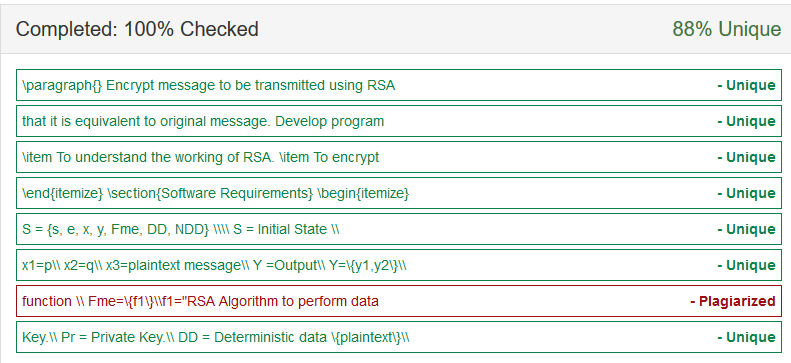
\includegraphics[width=\textwidth]{rsa}
\section{Output}
\begin{verbatim}
-----------------------------------------------
RSA output


Enter Message : 
123
P : 179
Q : 13
2327
Cipher : 301
Plaintext : 123
---------------------------------------------
\end{verbatim}
\end{document}


 

 
